\section{Segmented Sum/Scan Algorithm}

\subsection{Logical Step of SpMV}
\begin{frame}
	\frametitle{Logical Step of SpMV}
	\begin{enumerate}
		\item Read data value arrays and multiply them with the coresponding
			vector values indexed by the col\_index array.
		\item Perform a segmented scan by using the bit flag array from 
			BCCOO/BCCOO+ format.
		\item Write back result to global memory.
	\end{enumerate}
\end{frame}

\subsection{Segmented Scans}
\begin{frame}
	\frametitle{Segmented Scans}
	\begin{align*}
	\text{Input} 		&= [3, 2, 0, 2, 1, 0, 4, 2, 4, 3, 2, 2, 0, 1, 3, 1] \\
	\text{Bit Flag} 	&= [1, 1, 1, 1, 0, 1, 0, 1, 1, 0, 1, 1, 1, 1, 1, 0] \\ 
	\text{Start Flag} 	&= [1, 0, 0, 0, 0, 1, 0, 1, 0, 0, 1, 0, 0, 0, 0, 0] \\
	\text{Result}		&= [3, 5, 5, 7, \underline{8}, 0, \underline{4}, 2, 
		6, \underline{9}, 2, 4, 4, 5, 8, \underline{9}]
	\end{align*}
	\begin{figure}
		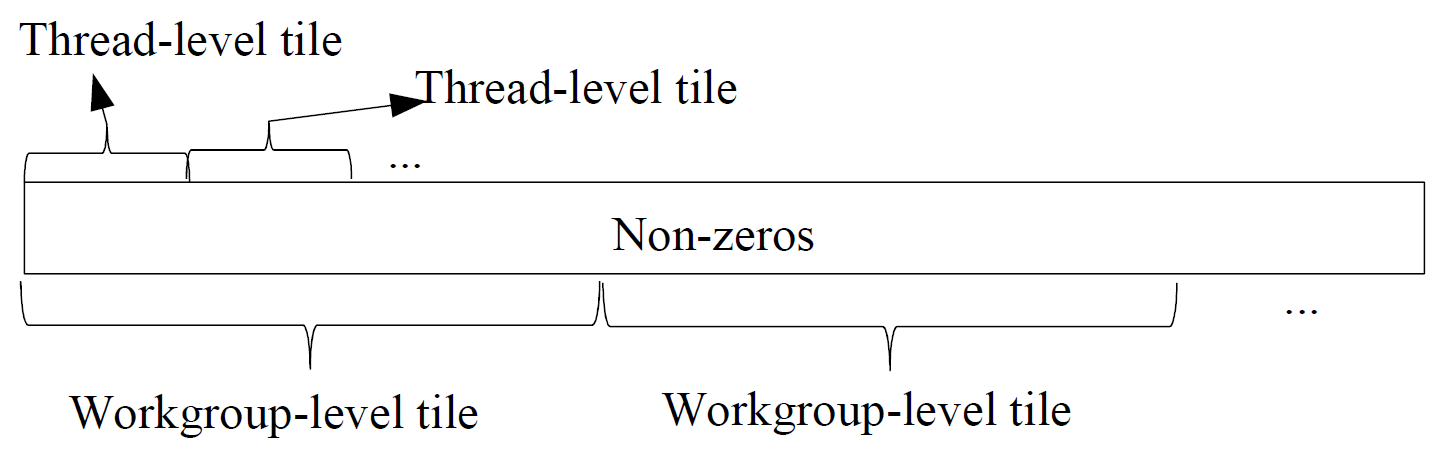
\includegraphics[scale=0.2]{figure/fig1-workload.png}
	\end{figure}
\end{frame}

\subsection{Matrix-based Segmented Sum/Scan}
\begin{frame}
	\frametitle{Matrix-based Strategy 1}
	\begin{itemize}
		\item Create \lstinline{intermediate_sums} in shared memory.
		\item If the lengths of segments are small, this strategy
			works well.
	\end{itemize}
\end{frame}
\begin{frame}
	\frametitle{Matrix-based Strategy 1 Example}
	\begin{figure}
		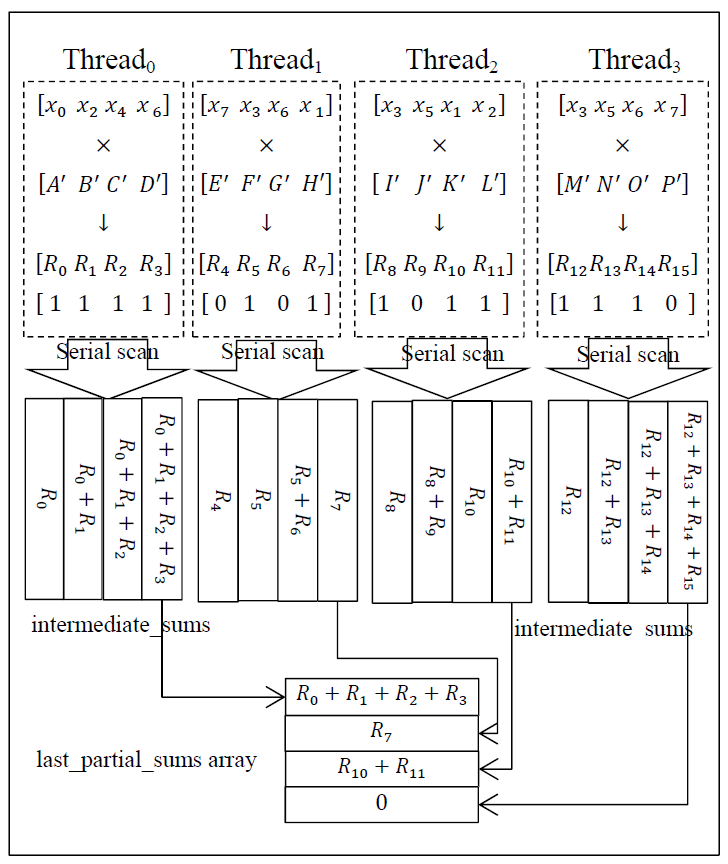
\includegraphics[scale=0.25]{figure/fig2-strategy1.png}
	\end{figure}
\end{frame}

\begin{frame}
	\frametitle{Matrix-based Strategy 2}
	\begin{itemize}
		\item Create result cache to store segmented sums.
		\item If the lenghts of segments are long, this strategy
			writes efficient-memory when we store result cache to
			global memory.
	\end{itemize}
\end{frame}
\begin{frame}
	\frametitle{Matrix-based Strategy 2 Example}
	\begin{figure}
		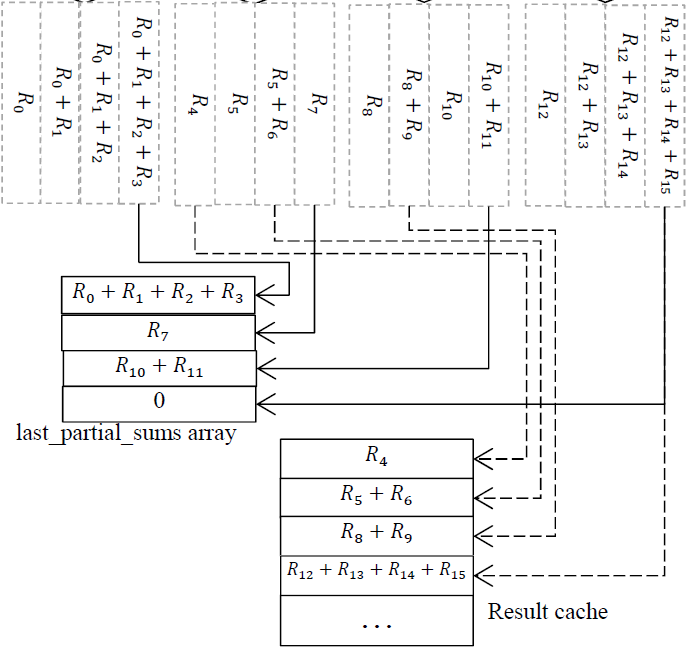
\includegraphics[scale=0.3]{figure/fig3-strategy2.png}
	\end{figure}
\end{frame}